\documentclass[10pt, twocolumn]{article}
%Gummi|065|=)
\title{\textbf{Stenio Garcia\\Federal University of Minas Gerais\\Theoretical Guide}}
\author{Marcos Paulo, Lucas Vazek $\&$ Thiago Silva}
\date{}

\usepackage[english]{babel}
\usepackage[utf8]{inputenc}
\usepackage{lscape}
\usepackage{fancyhdr}
\usepackage{rotating}
\usepackage{ragged2e}
\usepackage[a4paper, landscape, margin=0.8in]{geometry}
\usepackage{blindtext}
\usepackage{amsmath}
\usepackage{relsize}
\usepackage{graphicx}
\usepackage{float}
\usepackage{placeins}
\usepackage{enumitem}
\usepackage{booktabs}
\usepackage{array}
\usepackage{xcolor,colortbl}
\usepackage{tabu}


\setlength{\columnseprule}{0.4pt}
\setlength{\columnsep}{3em}
\graphicspath{ {img/} }
\restylefloat{table}

\newcommand{\mc}[2]{\multicolumn{#1}{c}{#2}}
\definecolor{Gray}{gray}{0.85}
\newcolumntype{a}{>{\columncolor{Gray}}c}


\begin{document}

\maketitle
\pagestyle{fancy}
\fancyhf{}
\rhead{Federal University of Minas Gerais - Stenio Garcia}
\lhead{Theoretical Guide}
\begin{flushleft}


%%%%%%%%%%%%%%%%%%%%%%%%%%%%%%%%%%%%%%%%%%%%%%%%%%%%%%%%%%%%%%%%%%%%%%%%%%%%%%%%
%																 			   %
%									SERIES									   %
%																			   %
%%%%%%%%%%%%%%%%%%%%%%%%%%%%%%%%%%%%%%%%%%%%%%%%%%%%%%%%%%%%%%%%%%%%%%%%%%%%%%%%
\section{Series}

$$\sum_{i=1}^{n} i = \frac{n(n+1)}{2}  \qquad  \sum_{i=1}^{n} i^{2} = \frac{n(n+1)(2n+1)}{6}  \qquad  \sum_{i=1}^{n} i^{3} = \frac{n^{2}(n+1)^{2}}{4}$$\\

Geometric Series:\\

$$a_n = a_1*c^{n-1} \qquad \sum_{i=0}^{n} c^{i} = \frac{c^{n+1}-1}{c-1}, \quad c \neq 1$$\\

$$\sum_{i=0}^{\infty} c^{i} = \frac{1}{1-c}, \quad \sum_{i=1}^{\infty} c^{i} = \frac{c}{1-c}, \quad |c| < 1$$\\

$$\sum_{i=0}^{n} ic^{i} = \frac{nc^{n+2} - (n+1)c^{n+1} + c}{(c-1)^{2}}, \quad c \neq 1$$

$$\sum_{i=0}^{\infty} ic^{i} = \frac{c}{(1-c)^{2}}, \quad |c| < 1$$



\vspace{50px}

%%%%%%%%%%%%%%%%%%%%%%%%%%%%%%%%%%%%%%%%%%%%%%%%%%%%%%%%%%%%%%%%%%%%%%%%%%%%%%%%
%																 			   %
%								IDENTITIES									   %
%																			   %
%%%%%%%%%%%%%%%%%%%%%%%%%%%%%%%%%%%%%%%%%%%%%%%%%%%%%%%%%%%%%%%%%%%%%%%%%%%%%%%%
\section{Identities}

\subsection{Combinatorics}

\begin{table}[H]
\setlength{\tabcolsep}{36pt}
\begin{tabular}{|c|c|}

\hline
$\mathlarger{\binom{n}{k} = \frac{n!}{(n-k)!k!}}$ & $\mathlarger{\sum_{k=0}^{n} \binom{n}{k}} = 2^n$ \\

\hline
$\mathlarger{\binom{n}{k} = \binom{n}{n - k}}$ &
$\mathlarger{\binom{n}{k} = \frac{n}{k}\binom{n-k}{m-k}}$ \\

\hline
$\mathlarger{\binom{n}{k} = \binom{n-1}{k} + \binom{n-1}{k-1}}$ &
$\mathlarger{\binom{n}{m}\binom{m}{k} = \binom{n}{k}\binom{n-k}{m-k}}$ \\

\hline
$\mathlarger{\sum_{k=0}^{n} \binom{r+k}{k} = \binom{r+n+1}{n}}$ &
$\mathlarger{\sum_{k=0}^{n} \binom{k}{k} = \binom{n+1}{m+1}}$ \\

\hline
$\mathlarger{\sum_{k=0}^{n} \binom{r}{k}\binom{s}{n-k} = \binom{r+s}{n}}$ & \\
\hline

\end{tabular}
\end{table}

\subsection{Newton's Binomial}

$$(x + y)^{n} = \sum_{k=0}^{n} \binom{n}{k} x^{n-k} y^{k} = \sum_{k=0}^{n} \binom{n}{k} x^{k} y^{n-k} $$\\
$$(1 + x)^{n} = \sum_{k=0}^{n} \binom{n}{k} x^{k}$$


\subsection{Catalan Numbers}

1, 1, 2, 5, 14, 42, 132, 429, 1430, 4862, 16796, 58786, 208012, 742900, 2674440, 9694845, 35357670, 129644790, 477638700, 1767263190, 6564120420, 24466267020, 91482563640, 343059613650, 1289904147324, 4861946401452, 18367353072152, 69533550916004, 263747951750360, 1002242216651368.\\

$$C_n = \frac{1}{n+1}\binom{2n}{n} = \frac{(2n)!}{(n+1)!n!} = \prod_{k=2}^{n} \frac{n+k}{k}, \quad n \geq 0$$\\


Applications:
\begin{itemize}
\item $C_n$ is the number of Dyck words of length 2n. A Dyck word is a string consisting of n Xs and n Ys such that no initial segment of the string has more Ys than Xs. For example, the following are the Dyck words of length 6.\\
XXXYYY  $\quad$  XYXXYY  $\quad$  XYXYXY  $\quad$  XXYYXY  $\quad$  XXYXYY


\item Re-interpreting the symbol X as an open parenthesis and Y as a close parenthesis, Cn counts the number of expressions containing n pairs of parentheses which are correctly matched.\\
((()))  $\qquad$  ()(())  $\qquad$  ()()()  $\qquad$  (())()  $\qquad$  ...


\item Successive applications of a binary operator can be represented in terms of a full binary tree. (A rooted binary tree is full if every vertex has either two children or no children.) It follows that $C_n$ is the number of full binary trees with n + 1 leaves:\\
\begin{center}
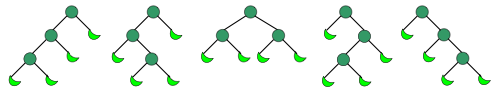
\includegraphics[scale=0.45]{Catalan_number_binary_tree_example.png}
\end{center}


\item $C_n$ is the number of monotonic lattice paths along the edges of a grid with n x n square cells, which do not pass above the diagonal. A monotonic path is one which starts in the lower left corner, finishes in the upper right corner, and consists entirely of edges pointing rightwards or upwards. Counting such paths is equivalent to counting Dyck words: X stands for ``move right" and Y stands for ``move up".
The following diagrams show the case n = 4:
\begin{center}
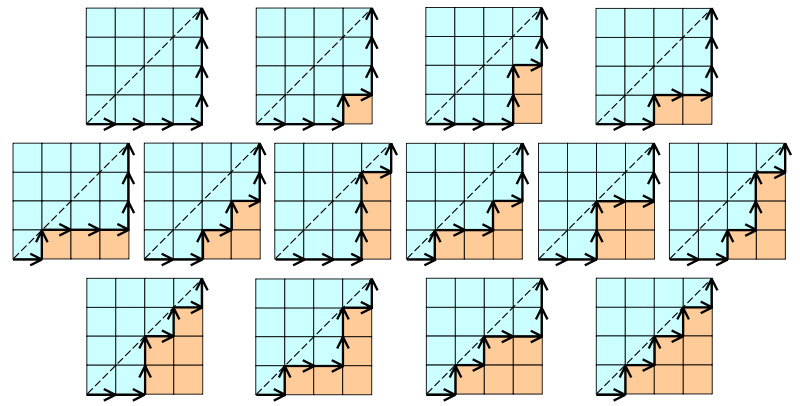
\includegraphics[scale=0.35]{Catalan_number_grid_example.png}
\end{center}


\item $C_n$ is the number of different ways a convex polygon with n + 2 sides can be cut into triangles by connecting vertices with straight lines (a form of Polygon triangulation). The following hexagons illustrate the case n = 4:
\begin{center}
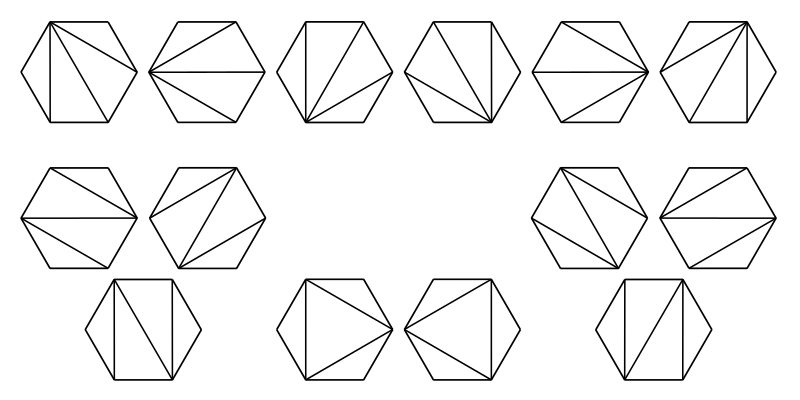
\includegraphics[scale=0.35]{Catalan-Hexagons-example.png}
\end{center}


\item $C_n$ is the number of rooted binary trees with n internal nodes (n + 1 leaves or external nodes). Illustrated in following Figure are the trees corresponding to n = 0,1,2 and 3. There are 1, 1, 2, and 5 respectively. Here, we consider as binary trees those in which each node has zero or two children, and the internal nodes are those that have children.
\begin{center}
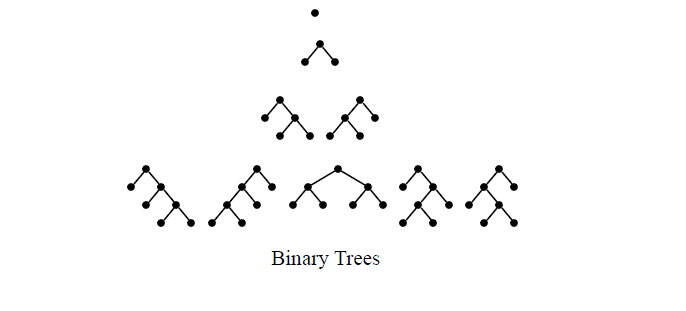
\includegraphics[scale=0.6]{Binary_Trees.png}
\end{center}


\item $C_n$ is the number of different ways n + 1 factors can be completely parenthesized (or the number of ways of associating n applications of a binary operator). For n = 3, for example, we have the following five different parenthesizations of four factors:\\
((ab)c)d  $\qquad$  (a(bc))d  $\qquad$  (ab)(cd)  $\qquad$  a((bc)d)  $\qquad$  a(b(cd))

\end{itemize}


%%%%%%%%%%%%%%%%%%%%%%%%%%%%%%%%%%%%%%%%%%%%%%%%%%%%%%%%%%%%%%%%%%%%%%%%%%%%%%%%
%																 			   %
%							  NUMBER THEORY									   %
%																			   %
%%%%%%%%%%%%%%%%%%%%%%%%%%%%%%%%%%%%%%%%%%%%%%%%%%%%%%%%%%%%%%%%%%%%%%%%%%%%%%%%
\section{Number Theory}

\textbf{Maximal Prime Gaps:}\\
For numbers until $10^9$ the maximal gap is 400.\\
For numbers until $10^{18}$ the maximal gap is 1500.\\[0.5cm]

\textbf{Number of prime numbers in intervals:}\\
There is aprox. $8*10^4$ primes between 1 e $10^6$.\\
There is aprox. $6*10^5$ primes between 1 e $10^7$.\\
There is aprox. $5*10^6$ primes between 1 e $10^8$.\\
There is aprox. $5*10^7$ primes between 1 e $10^9$.\\[0.5cm]



\textbf{Primes less than 1000:}\\
2$\quad$3$\quad$5$\quad$7$\quad$11$\quad$13$\quad$17$\quad$19$\quad$23$\quad$29$\quad$31$\quad$37\\

41$\quad$43$\quad$47$\quad$53$\quad$59$\quad$61$\quad$67$\quad$71$\quad$73$\quad$79$\quad$83$\quad$89\\

97$\quad$101$\quad$103$\quad$107$\quad$109$\quad$113$\quad$127$\quad$131$\quad$137$\quad$139$\quad$149$\quad$151\\

157$\quad$163$\quad$167$\quad$173$\quad$179$\quad$181$\quad$191$\quad$193$\quad$197$\quad$199$\quad$211$\quad$223\\

227$\quad$229$\quad$233$\quad$239$\quad$241$\quad$251$\quad$257$\quad$263$\quad$269$\quad$271$\quad$277$\quad$281\\

283$\quad$293$\quad$307$\quad$311$\quad$313$\quad$317$\quad$331$\quad$337$\quad$347$\quad$349$\quad$353$\quad$359\\

367$\quad$373$\quad$379$\quad$383$\quad$389$\quad$397$\quad$401$\quad$409$\quad$419$\quad$421$\quad$431$\quad$433\\

439$\quad$443$\quad$449$\quad$457$\quad$461$\quad$463$\quad$467$\quad$479$\quad$487$\quad$491$\quad$499$\quad$503\\

509$\quad$521$\quad$523$\quad$541$\quad$547$\quad$557$\quad$563$\quad$569$\quad$571$\quad$577$\quad$587$\quad$593\\

599$\quad$601$\quad$607$\quad$613$\quad$617$\quad$619$\quad$631$\quad$641$\quad$643$\quad$647$\quad$653$\quad$659\\

661$\quad$673$\quad$677$\quad$683$\quad$691$\quad$701$\quad$709$\quad$719$\quad$727$\quad$733$\quad$739$\quad$743\\

751$\quad$757$\quad$761$\quad$769$\quad$773$\quad$787$\quad$797$\quad$809$\quad$811$\quad$821$\quad$823$\quad$827\\

829$\quad$839$\quad$853$\quad$857$\quad$859$\quad$863$\quad$877$\quad$881$\quad$883$\quad$887$\quad$907$\quad$911\\

919$\quad$929$\quad$937$\quad$941$\quad$947$\quad$953$\quad$967$\quad$971$\quad$977$\quad$983$\quad$991$\quad$997\\[0.5cm]


\textbf{Other primes:}\\
The largest prime smaller than $10$   $\quad$  is 7.\\
The largest prime smaller than $10^2$    $\,$  is 97.\\
The largest prime smaller than $10^3$    $\,$  is 997.\\
The largest prime smaller than $10^4$    $\,$  is 9973.\\
The largest prime smaller than $10^5$    $\,$  is 99991.\\
The largest prime smaller than $10^6$    $\,$  is 999983.\\
The largest prime smaller than $10^7$    $\,$  is 9999991.\\
The largest prime smaller than $10^8$    $\,$  is 99999989.\\
The largest prime smaller than $10^9$    $\,$  is 999999937.\\
The largest prime smaller than $10^{10}$       is 9999999967.\\
The largest prime smaller than $10^{11}$ $\,$  is 99999999977.\\
The largest prime smaller than $10^{12}$ $\,$  is 999999999989.\\
The largest prime smaller than $10^{13}$ $\,$  is 9999999999971.\\
The largest prime smaller than $10^{14}$ $\,$  is 99999999999973.\\
The largest prime smaller than $10^{15}$ $\,$  is 999999999999989.\\
The largest prime smaller than $10^{16}$ $\,$  is 9999999999999937.\\
The largest prime smaller than $10^{17}$ $\,$  is 99999999999999997.\\
The largest prime smaller than $10^{18}$ $\,$  is 999999999999999989.\\[0.5cm]

\textbf{Random Primes}\\
1000000009 $\quad$ 1000000021 $\quad$ 1000000033 $\quad$ 1000000087 $\quad$ 1000000093
1000000097 $\quad$ 1000000103 $\quad$ 1000000123 $\quad$ 1000000181 $\quad$ 1000000207
1000000223 $\quad$ 1000000241 $\quad$ 1000000271 $\quad$ 1000000289 $\quad$ 1000000297
1000000321 $\quad$ 1000000349 $\quad$ 1000000363 $\quad$ 1000000403 $\quad$ 1000000409
2000003273 $\quad$ 2000003281 $\quad$ 2000003293 $\quad$ 2000003303 $\quad$ 2000003333
2000003351 $\quad$ 2000003353 $\quad$ 2000003359\\[0.5cm]



\textbf{Metodo de Newton}\\
$$x_{n+1} = x_n - \frac{f(x_n)}{f'(x_n)}$$
\begin{itemize}
\item O numero de casas decimais corretas, em media, dobra a cada iteracao. ( Em caso de duvida, default=30 ).
\end{itemize}

\vspace{0.5cm}

\textbf{Metodo dos Quadrados Minimos}\\
Queremos estimar valores de determinada variável $y$. Para isso, consideramos os valores de outra variavel $x$ que acreditamos ter poder de explicação sobre $y$ conforme a fórmula:
$$y = \alpha + \beta x + \epsilon$$
\begin{itemize}
\item $\alpha$: Parametro do modelo chamado de constante (porque não depende de $x$).
\item $\beta$: Parametro do modelo chamado de coeficiente da variavel $x$.
\item $\epsilon$:  Erro - representa a variação de $y$ que nao eh explicada pelo modelo.
\end{itemize}
Temos tambem uma base de dados com $n$ valores observados de $y$ e $x$. Ao fazer a estimativa de $\alpha$, $\beta$, e $\epsilon$, mudamos a notação de algumas variáveis:\\
$\alpha \, \rightarrow \, $ a.\\
$\beta \, \rightarrow \, $ b.\\
$\epsilon \, \rightarrow \, $ e.\\

Desse modo, ao estimar o modelo usando a base de dados, estamos estimando, na verdade:
$$y_i = a + bx_i + e_i$$
onde $i$ indica cada uma das $n$ observacoes da base de dados e $e$ passa a ser chamado de residuo, ao inves de erro.
O metodo dos minimos quadrados minimiza a soma dos quadrado dos residuos, ou seja, minimiza $\sum_{i=1}^{n} e_i^{2}$. Minimizando S(a, b) = $\sum_{i=1}^{n} (y_i - a - bx_i)^{2}$ temos que:\\
$$a = \bar{y} - b\bar{x}$$
$$b = \frac{\sum_{i=1}^{n} x_i (y_i - \bar{y})}{\sum_{i=1}^{n} x_i(x_i - \bar{x})} = \frac{\sum_{i=1}^{n} (x_i-\bar{x})(y_i - \bar{y})}{\sum_{i=1}^{n} (x_i - \bar{x})^{2}}$$
onde $\bar{y}$ eh a media amostral de $y$ e $\bar{x}$ eh a media amostral de $x$.\\[0.5cm]


\textbf{Funcao de Ackermann-Peter}\\
$$
A(m, n) =
\begin{cases}
n+1                  \; \quad \qquad \qquad \qquad \qquad se \quad m=0\\
A(m-1, 1)            \ \; \qquad \qquad \qquad se \quad m > 0 \quad e \quad n=0.\\
A(m-1, A(m, n-1))    \qquad se \quad m > 0 \quad e \quad n > 0.
\end{cases}
$$

\begin{itemize}
\item A(4, 2) tem 19729 digitos.
\end{itemize}


{\tabulinesep=1.2mm
\begin{tabu}[H]{|a|c|c|c|}

\hline
m$\backslash$n & 0 & 1 & 2\\

\hline
0 & 1 & 2 & 3\\

\hline
1 & 2 & 3 & 4\\

\hline
2 & 3 & 5 & 7\\

\hline
3 & 5 & 13 & 29\\

\hline
4 & 13 = $2^{2^{2}} \, - \, 3$  & 65533 = 2**3 - 3 & $2^{65536} \, - \, 3$ = 2**4 -3\\ \hline

\end{tabu}}


{\tabulinesep=1.2mm
\begin{tabu}[H]{|a|c|c|c|}

\hline
m$\backslash$n & 3 & 4 & n \\

\hline
0 & 4 & 5 & $n+1$ \\

\hline
1 & 5 & 6 & $n+2 = 2 + (n+3) - 3$\\

\hline
2 & 9 & 11 & $2n + 3 = 2(n+3) - 3$\\

\hline
3 & 61 & 125 & $2^{n+3} - 3$\\

\hline
4 & $2^{2^{2^65536}} \, - \, 3 =$ 2**5 - 3 & 2**6 - 3 & 2**(n+	2) - 3 \\ \hline

\end{tabu} }

Obs.: 2**n = $2^{2^{...}}$ 2, elevado a 2, elevado a 2... n vezes.\\
Ex.: 2**1 = $2^2$ $\quad$;$\quad$ 2**2 = $2^{2^{2}}$\\[0.5cm]

\textbf{Numeros de Mersenne}\\
$$\mathcal{M}(n) = 2^{n} - 1$$
onde $n$ eh um inteiro nao-negativo. Os numeros da forma $\mathcal{M}(n)$ sao conhecidos como numeros de Mersenne.\\
Um numero eh chamado de perfeito  se eh igual a metade da soma de todos os seus divisores positivos. Por exemplo, os divisores de 6 sao 1, 2, 3 e 6. Somando estes numeros obtemos:
$$1+2+3+6 = 12 = 2*6$$
Logo 6 eh perfeito. Em comparacao, nenhum primo eh perfeito. Todos os perfeitos pares sao da forma $2^{n-1}2(2^n - 1)$ com $2^n - 1$ primo. Assim, para achar os perfeitos pares basta achar os primos de Mersenne. Ninguem sabe se existem ou nao numeros perfeitos impares.
\begin{itemize}
\item Se $n$ eh um inteiro composto, entao $\mathcal{M}(n)$ eh composto.
\end{itemize}
\vspace{0.5cm}


\textbf{Teoremas de Fermat}\\
Seja $P$ um numero primo e $a$ um numero inteiro, entao:
$$a^p \equiv a \; (mod \; p)$$
$$a^{p-1} \equiv 1 \; (mod \; p)$$

\textbf{Lema:} Seja $p$ um numero primo e $a$ e $b$ inteiros. Entao:
$$(a+b)^{p} = a^{p} + b^{p} \; (mod \; p)$$

\textbf{Lema:} Seja $p$ um numero primo e $a$ inteiro. Entao, O inverso de a mod p eh $a^{p-2}$:
$$inv(a) \equiv a^{p-2} \; (mod \; p)$$




%%%%%%%%%%%%%%%%%%%%%%%%%%%%%%%%%%%%%%%%%%%%%%%%%%%%%%%%%%%%%%%%%%%%%%%%%%%%%%%%
%																 			   %
%								GEOMETRY									   %
%																			   %
%%%%%%%%%%%%%%%%%%%%%%%%%%%%%%%%%%%%%%%%%%%%%%%%%%%%%%%%%%%%%%%%%%%%%%%%%%%%%%%%
\section{Geometry}

\textbf{Conversao - angulos:}\\
$\qquad$ De radiano para grau:\\
$\qquad \qquad$ grau = radiano*(180/PI)\\
$\qquad$ De grau para radiano:\\
$\qquad \qquad$ radiano = grau*(PI/180)\\[0.5cm]

\textbf{Teorema de Herao}\\
A area de um triângulo pode ser dada por: A = $\sqrt{s\,(s-a)\,(s-b)\,(s-c)}$ em que $s$ representa o semi-perimetro do triângulo e $a$, $b$ e $c$ são os comprimentos de seus tres lados.\\[0.5cm]

\textbf{Central Angle}\\
Let $\phi_1$, $\lambda_1$ and $\phi_2$, $\lambda_2$ be the geographical latitude and longitude of two points 1 and 2, and $\Delta\phi$, $\Delta\lambda$ their absolute differences; then $\Delta\sigma$, the central angle between them, is given by the spherical law of cosines: $\Delta\sigma = arccos(sin\phi_1 \, sin\phi_2 + cos\phi_1 \, cos\phi_2 cos\Delta\lambda).$ The distance $d$, i.e. the arc-length, for a sphere of radius $r$ and $\Delta\sigma$ given in $d = r\Delta\sigma$.\\[0.5cm]

\textbf{Condicao de Existencia de Poligonos}\\
- Generalizacao da desigualdade triangular\\
- Given a collection of positive numbers $r_1$,...,$r_n$, there exists a polygon in $R^{2}$ with the side-lengths $r_1$,...,$r_n$ if and only if for every $i$, $r_i \, \textless $  1/2 * ($r_1$ + ... + $r_n$)\\[0.5cm]

\textbf{Lei dos Cossenos} $\qquad a^{2} = b^{2} - c^{2} - 2\,b\,c\,cosA$\\
\textbf{Lei dos Senos} $\, \quad \qquad \frac{a}{sin A} = \frac{b}{sin B} = \frac{c}{sin C}$




%%%%%%%%%%%%%%%%%%%%%%%%%%%%%%%%%%%%%%%%%%%%%%%%%%%%%%%%%%%%%%%%%%%%%%%%%%%%%%%%
%																 			   %
%								PROBABILITY									   %
%																			   %
%%%%%%%%%%%%%%%%%%%%%%%%%%%%%%%%%%%%%%%%%%%%%%%%%%%%%%%%%%%%%%%%%%%%%%%%%%%%%%%%
\section{Probability}

\textbf{Expectation}
$$E[X] = \sum_{i=1}^{\infty} x_i$$

\textbf{Bayes Theorem}
$$P(A|B) = \frac{P(B|A) P(A)}{P(B)}$$

\subsection{Distributions}
\subsubsection{Binomial}

$$P(X = k) = \binom{n}{k}\,p^{k}(1-p)^{n-k} \qquad \qquad E[X] = n*p$$

\begin{itemize}
\item Calcula a probabilidade de ter $K$ sucessos em $n$ tentativas.
\end{itemize}



\subsubsection{Geometric}
\begin{itemize}
\item $X$ eh o numero de fracassos em uma sequencia de ensaios independentes de Bernoulli ate que o primeiro sucesso seja observado.$$P(X = k) = (1-p)^{k}p$$
\item Ou, se pensar que $X$ eh o numero de tentativas ate o primeiro acerto...
$$P(X = k) = (1-p)^{k-1}p$$
\end{itemize}


Expectation: $E[X] = 1/p$




%%%%%%%%%%%%%%%%%%%%%%%%%%%%%%%%%%%%%%%%%%%%%%%%%%%%%%%%%%%%%%%%%%%%%%%%%%%%%%%%
%																 			   %
%									GRAPHS									   %
%																			   %
%%%%%%%%%%%%%%%%%%%%%%%%%%%%%%%%%%%%%%%%%%%%%%%%%%%%%%%%%%%%%%%%%%%%%%%%%%%%%%%%
\section{Graphs}

\subsection{Random Graphs}

% 
% Exemplo de Grafo: GraphViz
% http://www.graphviz.org/doc/info/attrs.html
% 
% graph G
% {
%        node [margin=0, width=0.3, shape=circle, style=filled, label=""];
%        edge [len=1];
%        A -- B;
%        A -- C;
%        B -- D;
%        B -- E;
%        B -- C;
%        C -- E;
%        C -- F;
%        E -- F;
%        D -- E;
% }
%

\begin{table}[H]
\setlength{\tabcolsep}{36pt}
\centering
\renewcommand{\arraystretch}{0.5}% Spread rows out...
\begin{tabular}{>{\centering}m{1in} >{\centering\arraybackslash}m{1in}}

\midrule
\raisebox{-\totalheight}{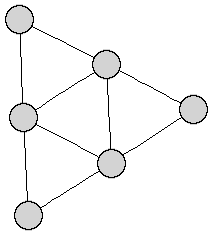
\includegraphics[angle=88, scale=0.3]{graph_sunlet_3.png}}
&
\raisebox{-\totalheight}{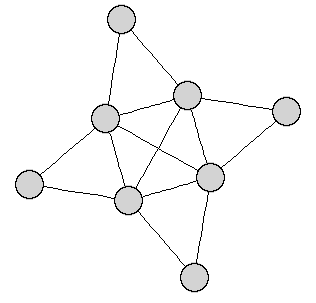
\includegraphics[scale=0.3]{graph_sunlet_4.png}}\\

\midrule
\raisebox{-\totalheight}{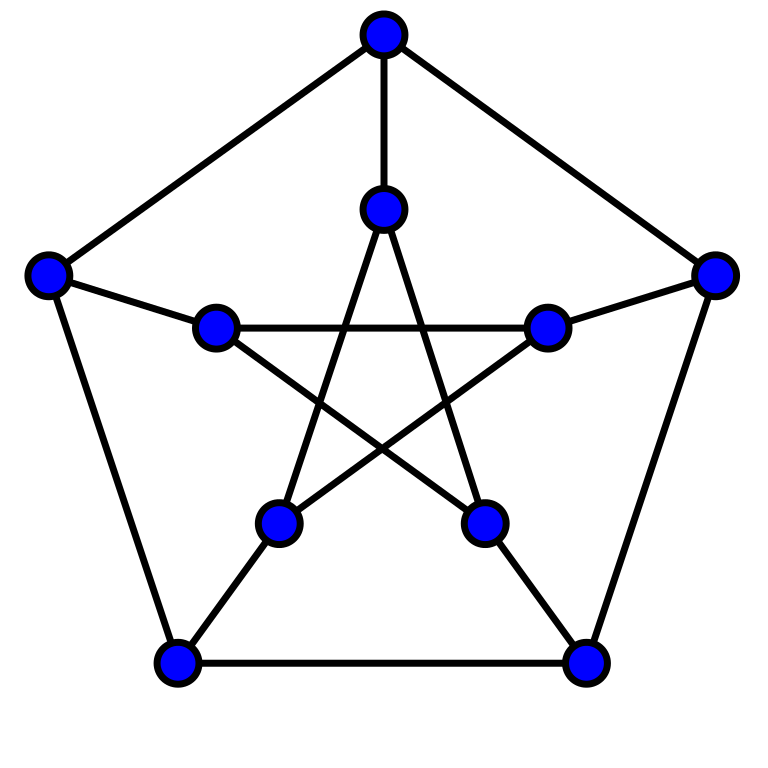
\includegraphics[scale=0.14]{Petersen.png}}
&
\raisebox{-\totalheight}{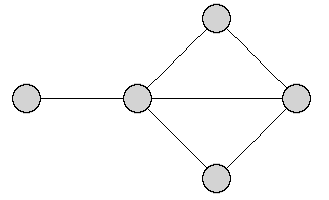
\includegraphics[scale=0.3]{random_graph1.png}}\\


\midrule
\raisebox{-\totalheight}{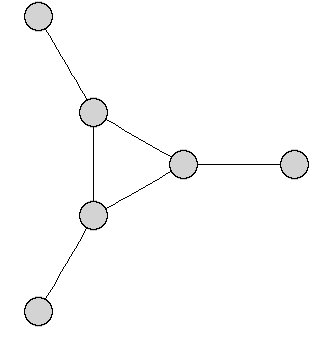
\includegraphics[angle=90, scale=0.3]{random_graph2.png}}
&
\raisebox{-\totalheight}{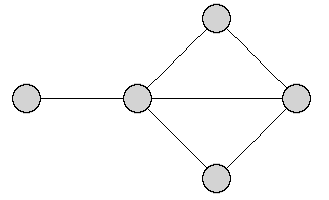
\includegraphics[scale=0.3]{random_graph1.png}}\\


\midrule
\raisebox{-\totalheight}{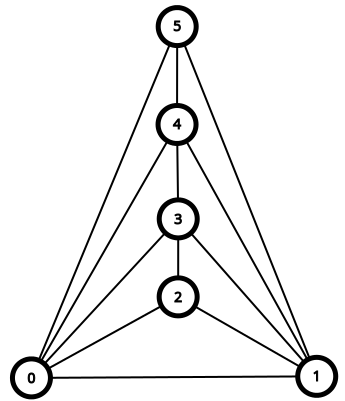
\includegraphics[scale=0.3]{random_graph3.png}}
&
\raisebox{-\totalheight}{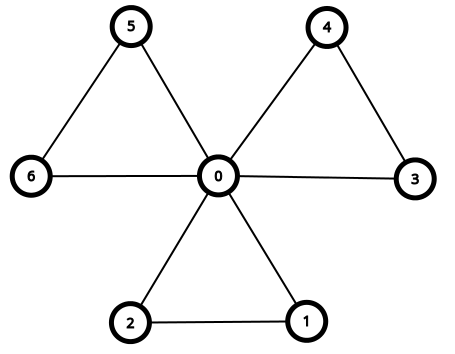
\includegraphics[scale=0.3]{random_graph4.png}}\\

\end{tabular}
\end{table}


\subsection{Graph Classes}
\subsubsection{Chordals}

\subsubsection{Line Graphs}

\subsubsection{Interval Graphs}

\subsubsection{Cactus}

\subsubsection{Perfect Graphs}

\subsubsection{Permutation Graphs}

\subsection{Theorems}





%%%%%%%%%%%%%%%%%%%%%%%%%%%%%%%%%%%%%%%%%%%%%%%%%%%%%%%%%%%%%%%%%%%%%%%%%%%%%%%%
%																 			   %
%									STRINGS									   %
%																			   %
%%%%%%%%%%%%%%%%%%%%%%%%%%%%%%%%%%%%%%%%%%%%%%%%%%%%%%%%%%%%%%%%%%%%%%%%%%%%%%%%
\section{Strings}

\begin{center}
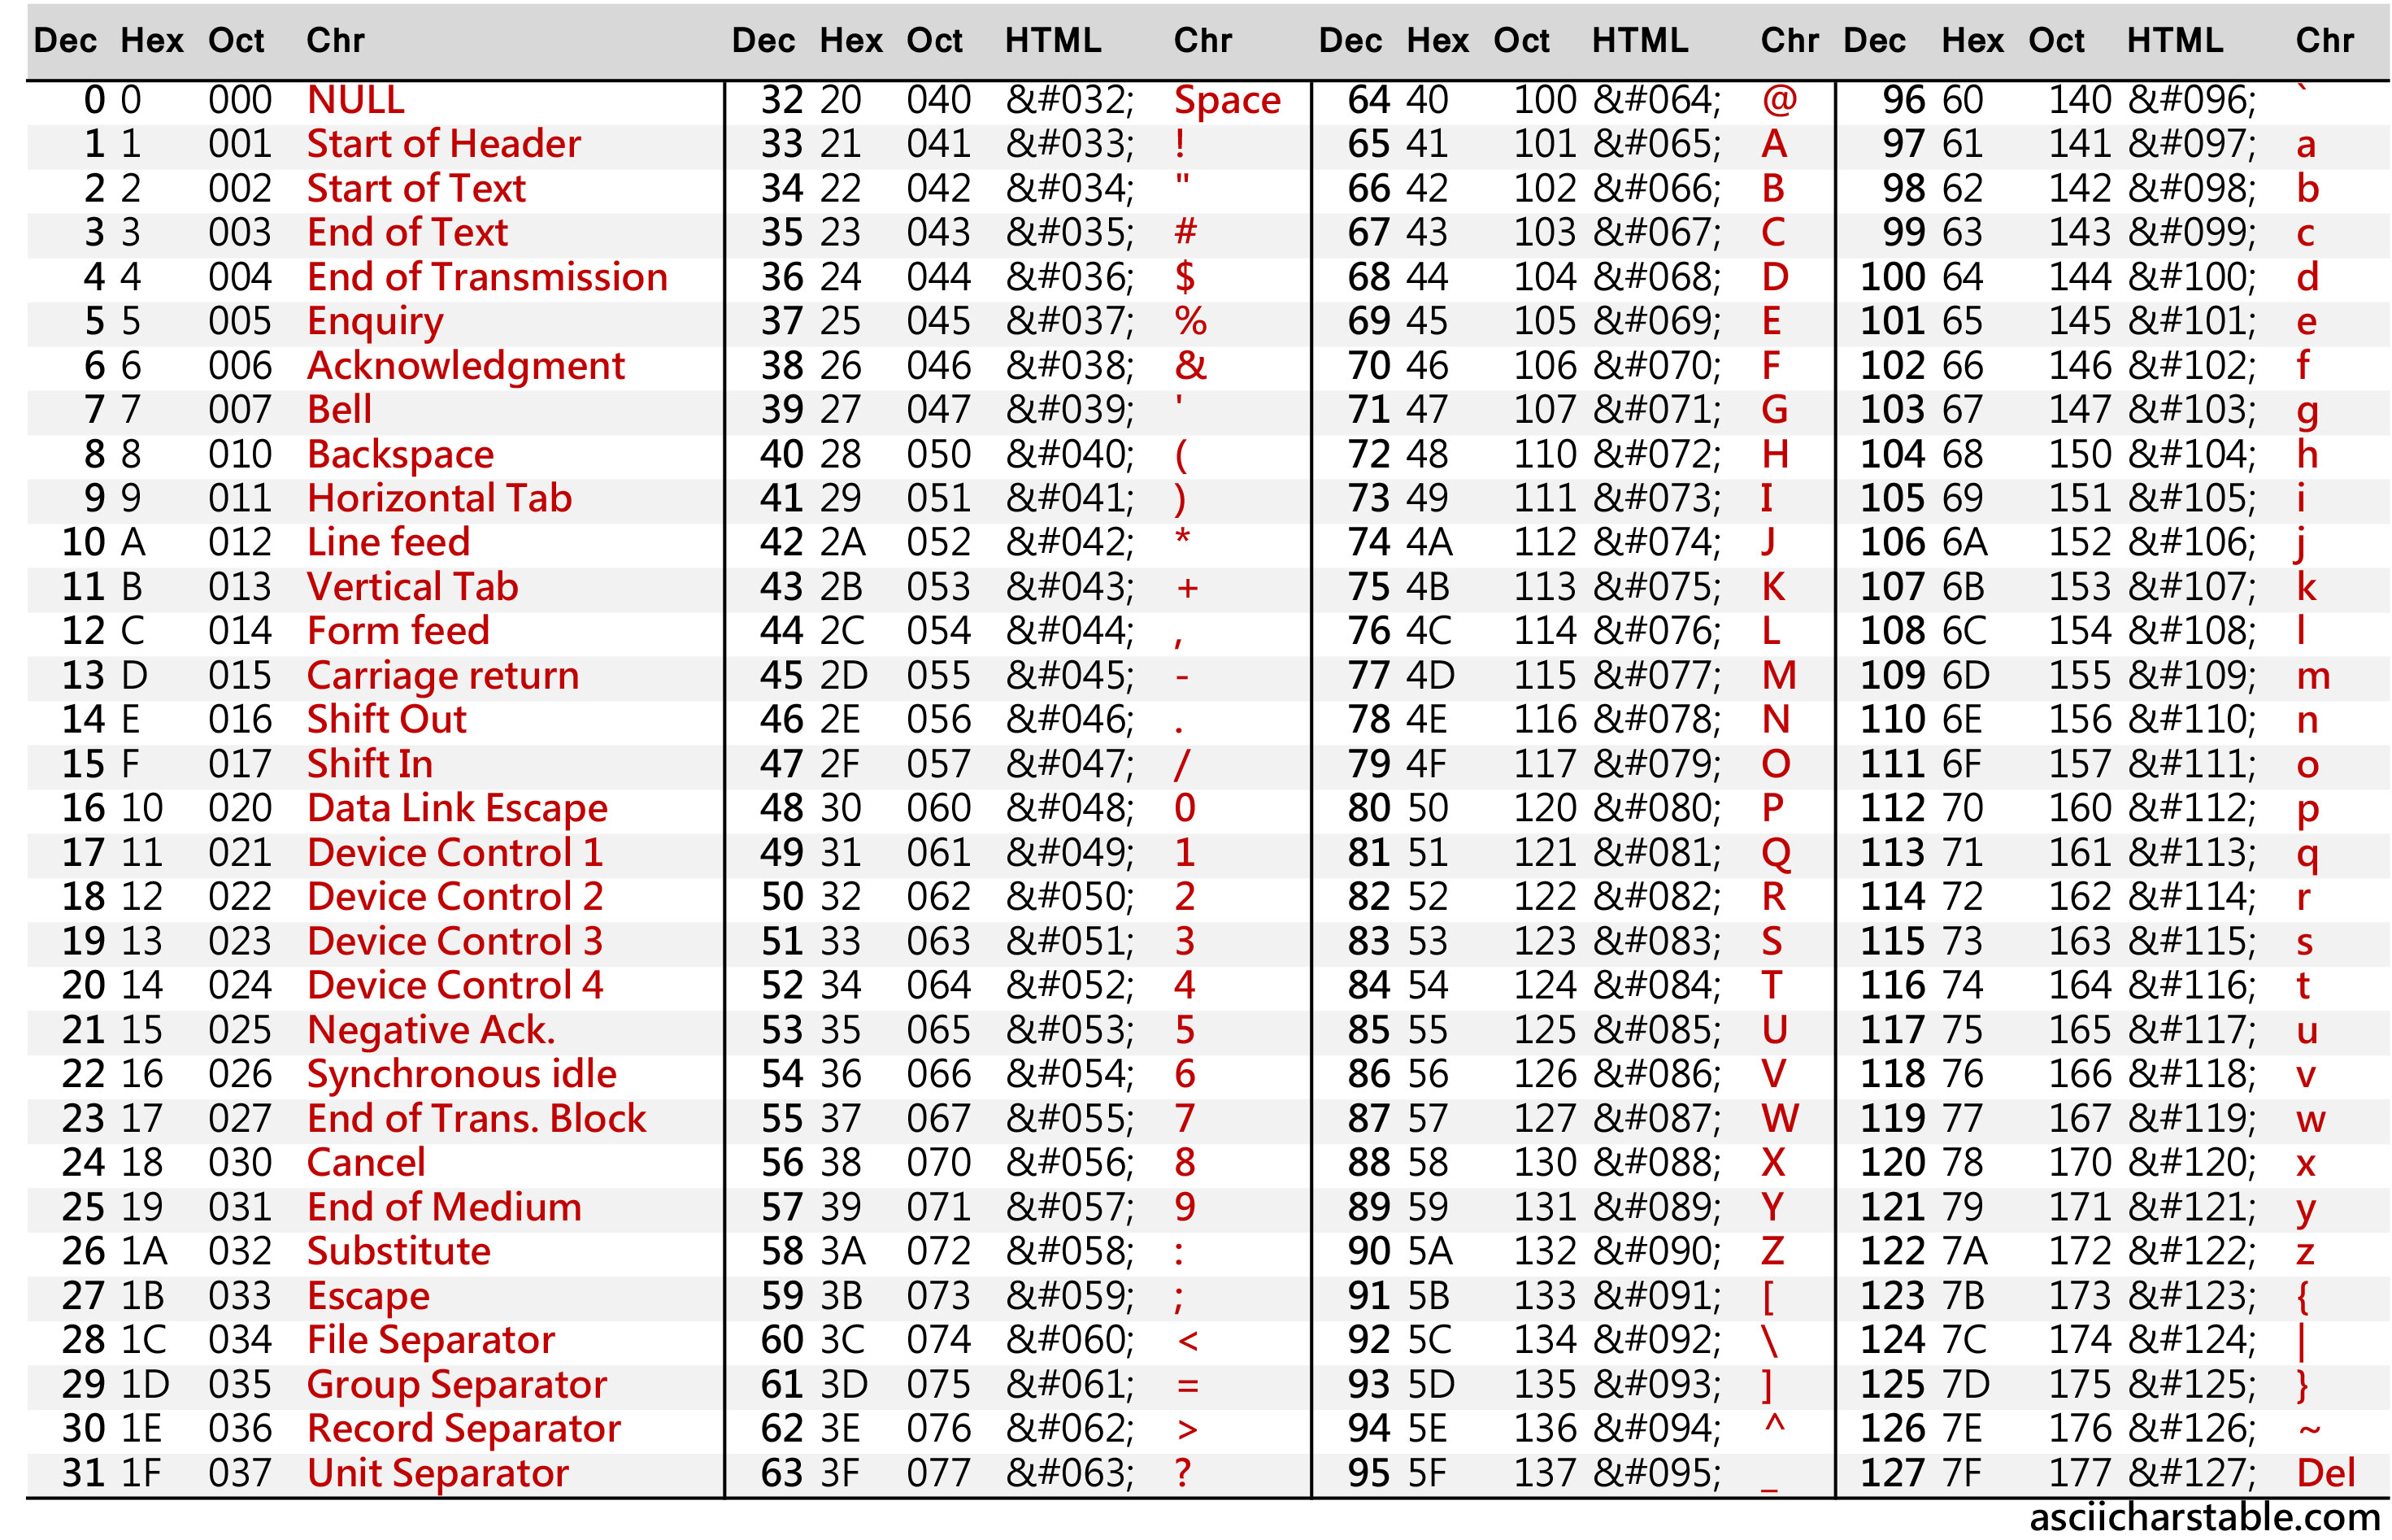
\includegraphics[scale=0.13]{ASCII-Table-wide.jpg}
\end{center}




\end{flushleft}
\end{document}